% \documentclass[CJKutf8, 10pt, handout]{beamer}
\documentclass[10pt]{beamer}
\usetheme[
%%% options passed to the outer theme
%    hidetitle,           % hide the (short) title in the sidebar
%    hideauthor,          % hide the (short) author in the sidebar
%    hideinstitute,       % hide the (short) institute in the bottom of the sidebar
%    shownavsym,          % show the navigation symbols
%    width=2cm,           % width of the sidebar (default is 2 cm)
     hideothersubsections,% hide all subsections but the subsections in the current section
%    hideallsubsections,  % hide all subsections
%    right                % right of left position of sidebar (default is right)
]{Aalborg}
  
% If you want to change the colors of the various elements in the theme,
% edit and uncomment the following lines.
% Change the bar and sidebar colors:
\setbeamercolor{Aalborg}{fg=black!20,bg=TJblue}
\setbeamercolor{sidebar}{bg=white}
% Change the color of the structural elements:
%\setbeamercolor{structure}{fg=red}
% Change the frame title text color:
%\setbeamercolor{frametitle}{fg=blue}
% Change the normal text color background:
\setbeamercolor{normal text}{bg=gray!6}
\usepackage{ctex} % 必须使用 ctex 宏包
\setCJKmainfont{STSong} % 全局中文用 Adobe Song Std 字体
%\usepackage{CJKutf8}
\usepackage{color}
\usepackage{graphicx}
\usepackage{fancybox}
\usepackage[utf8]{inputenc}
\usepackage[english]{babel}
\usepackage[T1]{fontenc}
% ... or whatever. Note that the encoding and the font should match.
% If T1 does not look nice, try deleting the line with the fontenc.
\usepackage{lmodern} %optional
\usepackage{listings}
\usepackage{wasysym}

%%%%%%%% User Specified Commands %%%%%%%%
\setbeamercolor{alerted text}{fg=red!2!green!35!blue}
\newenvironment{boxalertenv}{\begin{altenv}%
  {\usebeamertemplate{alerted text begin}\usebeamercolor[fg]
    {alerted text}\usebeamerfont{alerted text}\colorbox{bg}}
  {\usebeamertemplate{alerted text end}}{\color{.}}{}}{\end{altenv}}
\newcommand<>{\boxalert}[1]{{%
  \begin{boxalertenv}#2{#1}\end{boxalertenv}%
}}


\definecolor{listinggray}{gray}{0.9}
\definecolor{lbcolor}{rgb}{0.9,0.9,0.9}
\definecolor{TJblue}{rgb}{0.0469,0.2461,0.6016}



\def\hilite<#1>{%
  \temporal<#1>{\color{gray}}{\color{TJblue}}%
    {\color{black}}}

% colored hyperlinks
\newcommand{\chref}[2]{%
  \href{#1}{{\usebeamercolor[bg]{Aalborg}#2}}
}

%%%%%%%%%%%%%%%%%%%%%%%%%%%%%%%%%%%%%%%%%%%%%%%%%%%%%%%%%%%%%%%%%%%%%%%%%%%%%%%%%%%%%%%%%%%%%%
\lstset{
	language=C,
	captionpos=b,
	tabsize=4,
	frame=lines,
	keywordstyle=\color{blue},
	commentstyle=\color{darkgreen},
	stringstyle=\color{red},
	breaklines=true,
	showstringspaces=false,
	basicstyle=\footnotesize,
	emph={label}
	}

%%%%%%%% 设置字号 %%%%%%%%
\newcommand{\chuhao}{\fontsize{42pt}{\baselineskip}\selectfont}
\newcommand{\xiaochuhao}{\fontsize{36pt}{\baselineskip}\selectfont}
\newcommand{\yihao}{\fontsize{28pt}{\baselineskip}\selectfont}
\newcommand{\erhao}{\fontsize{21pt}{\baselineskip}\selectfont}
\newcommand{\xiaoerhao}{\fontsize{18pt}{\baselineskip}\selectfont}
\newcommand{\sanhao}{\fontsize{15.75pt}{\baselineskip}\selectfont}
\newcommand{\sihao}{\fontsize{14pt}{\baselineskip}\selectfont}
\newcommand{\xiaosihao}{\fontsize{12pt}{\baselineskip}\selectfont}
\newcommand{\wuhao}{\fontsize{10.5pt}{\baselineskip}\selectfont}
\newcommand{\xiaowuhao}{\fontsize{9pt}{\baselineskip}\selectfont}
\newcommand{\liuhao}{\fontsize{7.875pt}{\baselineskip}\selectfont}
\newcommand{\xiaoliuhao}{\fontsize{6.05pt}{\baselineskip}\selectfont}
\newcommand{\qihao}{\fontsize{5.25pt}{\baselineskip}\selectfont}

\AtBeginSection[]
{
\begin{frame}[shrink]
  \frametitle{目录}
  \tableofcontents[%
 		currentsection, % causes all sections but the current to be shown in a semi-transparent way.
% 		currentsubsection, % causes all subsections but the current subsection in the current section to ...
% 		hideallsubsections, % causes all subsections to be hidden.
 		hideothersubsections, % causes the subsections of sections other than the current one to be hidden.
% 		part=, % part number causes the table of contents of part part number to be shown
%		pausesections, % causes a \pause command to be issued before each section. This is useful if you
% 		pausesubsections, %  causes a \pause command to be issued before each subsection.
% 		sections={ overlay specification },
  ]
\end{frame}
}

\begin{document}


\title[工学硕士毕设答辩]% optional, use only with long paper titles
{\erhao 永磁同步电机伺服系统\\自抗扰控制研究\\[2ex]}

%\subtitle[OSS\ C\ SDK] %optional
%{OSS\ C\ SDK\ 简介}

\author[徐晨剑] % optional, use only with lots of authors
{
\textcolor[rgb]{0.00, 0.41, 0.66}{11111徐晨剑\inst{1} \and 王维\inst{2}\\[2ex]}
\textcolor[rgb]{0.00, 0.41, 0.66}{\texttt{\{\inst{1}haipingf, \inst{2}wangwei881116\}@gmail.com}}
% \href{mailto:haipingf@gmail.com}{{\tt haipingf@gmail.com}}
}

% - Give the names in the same order as they appear in the paper.
% - Use the \inst{?} command only if the authors have different
%   affiliation. See the beamer manual for an example

%specify some optional logos
% placed in the upper left/right corner
\pgfdeclareimage[height=1.0cm]{mainlogo}{1.png} 
\logo{\pgfuseimage{mainlogo}}
% placed in the lower left/right corner if the \pgfuseimage{minilogo} command is
% uncommented in the \institute command below.
\pgfdeclareimage[height=0.3cm]{minilogo}{2.png} 

\institute[
  {\pgfuseimage{minilogo}}\\ %insert a company or department logo
  College of Electronics and Information Engineering\\
  Tongji University, Shanghai
] % optional - is placed in the bottom of the sidebar on every slide
{%
\textcolor[rgb]{0.07, 0.31, 0.60}{
  \wuhao 同1111济大学\\[2ex]
  \xiaowuhao 电子与信息工程学院, 上海}
  
  % there must be an empty line above this line - otherwise some unwanted space is added
  % between the university and the country (I do not know why;( )
}
% \date{\today}
\date{\textcolor[rgb]{0.07, 0.31, 0.60}{\today}}

% the titlepage
% the plain option removes the sidebar and header from the title page
\begin{frame}[plain] 
  \titlepage
\end{frame}
%%%%%%%%%%%%%%%%

%%对页数、章数、小结数有改动时,编译前请先将下面这句注销掉,编译生成后,再取消注销,再次编译
% TOC


%\begin{frame}{总览}{}
%  \tableofcontents
%\end{frame}
%%%%%%%%%%%%%%%%%%%%%%%%%%%%%%%%%%%%%%%%%%%%%%%%%%%%%%%%%%%%
\section{绪论}
%%%%%%%%%%%%%%%%
\subsection{课题背景与研究意义}

%%%%%%%%%%%%%%%%%%%%%%%%%%%%%%%%%%%%%%%%%
\begin{frame}{课题背景与研究意义}{}
  \begin{itemize}
	\hilite<1> \item{\sanhao 近距离体验云计算魅力}
  \end{itemize}
  \begin{itemize}
	\hilite<2> \item{\sanhao 在实战中提高个人能力}
  \end{itemize}
\begin{itemize}
	\hilite<3> \item{\sanhao 证明自己,回报开源社区}
  \end{itemize}
\begin{itemize}
	\hilite<4> \item{\sanhao 奖品丰厚,\smiley}
  \end{itemize}
\end{frame}
%%%%%%%%%%%%%%%%
\subsection{国内外研究现状}
\begin{frame}{国内外研究现状}{}
  \begin{columns}[t]
	\column{0.5\textwidth}
	 % \begin{center} \includegraphics[height=3cm]{U200714587.png} \end{center} %加图片
	  \begin{block}{傅海平,男} \xiaoliuhao 2011年毕业于华中科技大学,同年进入中国科学院计算技术研究所,硕士在读,宅,喜静,性格随和,崇尚开源与自由,
	  典型的GNU/Linux控,Vim 重度患者,热爱技术与生活。\end{block}
	\pause
	\column{0.5\textwidth}
	 % \begin{center} \includegraphics[height=3cm]{U200714718.png} \end{center}
	  \begin{block}{王\ 维,男} \xiaoliuhao 2011年毕业于华中科技大学,同年进入中国科学院计算技术研究所,硕士在读,兴趣广泛,性格开朗,喜欢音乐、运动、旅游,热爱技术。 \end{block}
  \end{columns}
\end{frame}
%%%%%%%%%%%%%%%%
\subsection{论文主要研究内容}
\begin{frame}{论文主要研究内容}{}
  \begin{itemize}
    \hilite<1> \item OSSC 为阿里云开放存储服务(OSS)提供了一套完整易用的 C SDK,并且实现了面向对象的调用方式。
	\hilite<2> \item OSSC 实现了 OSS 开放接口规范中所描述的所有功能,包括 Bucket,Object,Multipart Upload 和 Group Object 四大类操作。
	\hilite<3> \item 此外还提供诸如多线程断点上传,支持多种压缩算法的文件(或内存块)上传和下载,文件夹同步等高级特性。
	\hilite<4> \item OSSC 良好的接口设计能够大大简化其他用户的编程工作,其他用户可以通过 OSSC 提供的 API 更方便地访问阿里云开放存储服务。
  \end{itemize}
\end{frame}
%%%%%%%%%%%%%%%%%%%%%%%%%%%%%%%%%%%%%%%%%%%%%%%%%%%%%%%%%%%%
\section{永磁同步电机控制模型}
%%%%%%%%%%%%%%%%
\subsection{永磁同步电机数学模型}
\begin{frame}{永磁同步电机数学模型}
  \begin{block}{}{\alert<1>{OSSC 提供了《阿里云开放存储服务 OSS》中的四大类基本接口,分别是:}}
  \end{block}
  \pause
  \begin{enumerate}
	\hilite<2> \item {\tt Bucket 操作}
    \hilite<3> \item {\tt Object 操作}
    \hilite<4> \item {\tt Multipart Upload 操作}
    \hilite<5> \item {\tt Object Group操作}
  \end{enumerate}
\end{frame}
%%%%%%%%%%%%%%%%
\begin{frame}{基本功能介绍}
  \begin{block}{}{
	\alert<1>{访问阿里云开放存储服务的入口“类”是 \emph{oss\_client\_t},
	与此对应的所有函数均以 \emph{client\_} 前缀开头,
	并且第一个参数都是指向 \emph{client} 结构的指针。例如:}}
  \end{block}
  \pause
  \begin{itemize}
	\hilite<2> \item {设置 Bucket 权限: }
	\hilite<3> \item {void client\_set\_bucket\_acl(
                 \textcolor[rgb]{1.00, 0.0, 0.0}{oss\_client\_t *client},
			               const char *bucket\_name,
			               const char *acl,
			               unsigned short *retcode);}
  \end{itemize}
\end{frame}
%%%%%%%%%%%%%%%%
\begin{frame}{基本功能介绍}
  \begin{block}{}{
	\alert<1>{\emph{client\_} 函数簇出错信息处理}}
  \end{block}
  \pause
  \begin{itemize}
	\hilite<2> \item {void client\_set\_bucket\_acl(
	                       oss\_client\_t *client,
			               const char *bucket\_name,
			               const char *acl,
						   \textcolor[rgb]{1.00, 0.0, 0.0}{unsigned short *retcode);}}
    \hilite<3> \item {\emph{client\_} 函数簇中的每个函数的最后一个参数是 \emph{\tt unsigned short *} 类型。}
	\hilite<4> \item {如果不需要获取出错信息,可以向该参数传递 \emph{\tt NULL}}
	\hilite<5> \item {否则需要传递一个 \emph{\tt unsigned short} 类型存储单元地址。}
	\hilite<6> \item {函数返回后,出错信息保存在 \emph{\tt retcode} 指向的内存单元中。}
	\hilite<7> \item {最后调用{\tt oss\_why()\onslide<7>{\footnote{\onslide<7>{0.1.6 新增,旧版本为 {\tt oss\_get\_error\_message\_from\_retcode()}}}} 获取具体(human-readable)出错信息。}}
  \end{itemize}
\end{frame}
%%%%%%%%%%%%%%%%
\subsection{空间矢量脉宽调制}
\begin{frame}{空间矢量脉宽调制}
  OSSC 在 Ubuntu 12.04 上开发,我们测试了OSSC 在不同Linux 操作系统发行版的稳定性,以下是 OSSC 经过测试操作系统:
  \pause
\begin{itemize}[<+- | alert@+>]
    \item {\tt Ubuntu 12.04, 11.10, 11.04, 10.10, 10.04}
    \item {\tt CentOS 5.5}
    \item {\tt Fedora 15, 16, 17}
    \item {\tt openSUSE 12.2}
  \end{itemize}
\end{frame}
%%%%%%%%%%%%%%%%
\begin{frame}{编译与安装}
  \alert{OSSC 基于 \emph{\tt CMake} 构建,并依赖 \emph{\tt CURL} 库进行 HTTP 请求操作,
  此外不依赖其他第三方库,因此你只需要确保你的系统中安装了 \emph{\tt CMake} 和 \emph{\tt CURL} 库。}
  \pause
\begin{itemize}[<+- | alert@+>]
  \item {\tt 安装 CURL,\url{http://curl.haxx.se/download.html}}
  \item {\tt 下载 OSSC 源码并解压,进入到 build 目录,执行 cmake ../.}
  \item {\tt 编译和安装 make \&\& make install}
  \item {\tt OSSC默认安装在 /usr/local目录下,可以如下指定安装路径:}
  \item {\tt cmake -DCMAKE\_INSTALL\_PREFIX = /your-path ../.}
  \end{itemize}
\end{frame}
%%%%%%%%%%%%%%%%
\subsection{永磁同步电机伺服控制}
\begin{frame}{永磁同步电机伺服控制}{}
  \begin{block}{}{\alert<1>{OSSC 为开发者提供了丰富的文档和大量的示例\\}}\end{block}
  \pause
  \begin{itemize}[<+- | alert@+>]
    \item OSSC 的开发者文档位于 {\tt doc/html} 中,强烈建议开发者首先与读相关页面,加深对 OSSC 的理解。
	\item OSSC 目前提供的开发者手册包括《OSSC 介绍》,《OSSC 安装步骤》,《OSSC 编码规范》,《OSSC 实现原理》,《高级模块 Extra 库》,《API 使用示例》以及由 \emph{\tt Doxygen} 生成的 API 索引。
	\item 示例代码位于 {\tt example} 目录中,默认情况下,编译 OSSC 会为各个示例生成可执行文件,
		可执行文件位于 {\tt build/example} 目录中。
  \end{itemize}
\end{frame}
%%%%%%%%%%%%%%%%
\begin{frame}{开发者手册}{}
  \begin{center} 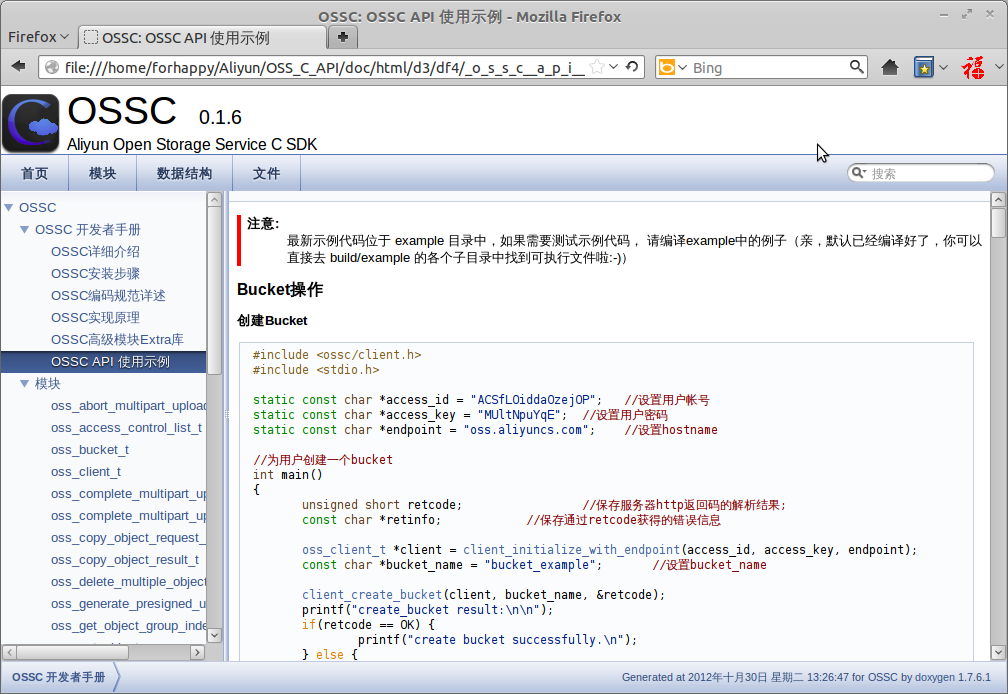
\includegraphics[width=1.0\textwidth]{ossc-api-example.png} \end{center}
\end{frame}
%%%%%%%%%%%%%%%%%%%%%%%%%%%%%%%%%%%%%%%%%%%%%%%%%%%%%%%%%%%%
\section{永磁同步电机自抗扰控制器}
%%%%%%%%%%%%%%%%
\subsection{自抗扰控制器理论}
\begin{frame}[fragile]{自抗扰控制器理论}{}
  \begin{block}{}{\alert<1>{OSSC 内置了多线程断点续传的功能\footnote{目前多线程只支持 \emph{\tt Pthread},所以为了不影响跨平台性,
	我们将该功能集成到 \emph{ossextra} 包中,在你的程序中需要设置链接参数 \emph{\tt -lossextra}}}}
  \end{block}
  \pause
  \lstset{language=C,basicstyle=\ttfamily,commentstyle=\ttfamily}
  \lstdefinestyle{Java}{delim=[il][\bfseries]{BB}}
  \definecolor{lightgray}{rgb}{.9,.9,.9}
  \lstset{backgroundcolor=\color{lightgray}}
  \begin{footnotesize}
    \begin{block}{}
      \begin{lstlisting}[language=C]
    extern void 
    client_extra_put_object(oss_client_t *client,
                const char *bucket_name,
                const char *key,
                const char *local_file,
                unsigned short *retcode);
	  \end{lstlisting}
    \end{block}
  \end{footnotesize}
\end{frame}
%%%%%%%%%%%%%%%%
\begin{frame}{多线程断点上传}{}
  \begin{block}{}{\alert<1>{多线程断点上传实现原理}}\end{block}
  \begin{itemize}
    \hilite<2> \item OSSC 实现了一个简洁的线程池,池中默认线程数目为 4。
	\hilite<3> \item{多线程上传过程中主线程会在当前目录下创建一个文件夹,
	用于保存 Upload ID 和已成功上传文件块的元信息,
	上传成功后该文件夹将被删除。}
	\hilite<4> \item 如果某次上传过程被中断,再次启动上传时不会重复上传先前已成功上传的文件块。
  \end{itemize}
  \pause
\end{frame}
%%%%%%%%%%%%%%%%
\subsection{永磁同步电机自抗扰控制}
\begin{frame}{永磁同步电机自抗扰控制}{}
  \begin{block}{}{\alert<1>{OSSC 为阿里云存储设计了一套可扩展的压缩文件格式,
	最多支持 256 种压缩算法,开发者可以实现自己的压缩方式,目前内置 LZ4,LZO 两种压缩算法。}}
  \end{block}
  \vskip 0.4cm
  \begin{block}{}{\alert<2>{为什么设计一套支持多种压缩算法的文件格式 ?}}
  \end{block}
  \begin{block}{}{\onslide<3>{\alert<3>{
	不同的压缩算法压缩比和压缩速率不同,压缩比越大,可能压缩速率越低,但是压缩后的文件更小,更适合网络传输;
	相反,压缩速率越快,可能压缩效果不是非常出色,但是可以近实时压缩。}}}
  \end{block}
\end{frame}
%%%%%%%%%%%%%%%%
\begin{frame}[fragile]{可扩展压缩文件格式}{}
  \begin{tiny}
  \begin{verbatim}
+---+---+---+---+---+---+---+---+
|"O"|"S"|"S"|"C"| V | A | F | L |   "OSSC": Magic Number;
+---+---+---+---+---+---+---+---+        V: Compressed File Version, Current Version 0x1
|           MD5[00-07]          |        A: Compression Algorithm, 0x1(LZ4), 0x2(LZO), ...
+---+---+---+---+---+---+---+---+        F: Flag, 0x1:Integrity Check, ...
|           MD5[08-15]          |        L: Header Length, Max Value 255
+---+---+---+---+---+---+---+---+ Optional: Optional Header, Not Used In Version 0x1
|       Optional(4 Bytes)       |
+---+---+---+---+---+---+---+---+--+                                                 
| Block  Length |               |  |                                                 
+---------------+               |  \                                                 
|                               |   X(Compressed Data Block 1)                       
|      Compressed Data          |  /                                                 
|                               |  |                                                 
+----------------+--------------+--+                                                 
| Block  Length  |              |  |                                                 
+----------------+              |  \                                                 
|                               |   X(Compressed Data Block 2)                       
|      Compressed Data          |  /                                                 
|                               |  |                                                 
+-------------------------------+--+                                                 
|                               |  |                                                 
|         Compressed            |  \                                                 
|            Data               |   X(Compressed Data Block 3 ~ (n - 1))             
|           Blocks              |  /                                                 
|                               |  |                                                 
+-------------------------------+--+                                                 
| Block  Length |               |  |                                                 
+---------------+               |  \                                                 
|                               |   X(Compressed Data Block n)                       
|      Compressed Data          |  /                                                 
|                               |  |                                                 
+-------------------------------+--+                                                 
  \end{verbatim}
  \end{tiny}
\end{frame}
%%%%%%%%%%%%%%%%
\begin{frame}[fragile]{可扩展压缩文件格式}{}
  \begin{block}{}{\alert<1>{OSSC 文件压缩、解压缩 API}}
  \end{block}
  \vskip 0.4cm
  \lstset{language=C,basicstyle=\ttfamily,commentstyle=\ttfamily}
  \lstdefinestyle{Java}{delim=[il][\bfseries]{BB}}
  \definecolor{lightgray}{rgb}{.9,.9,.9}
  \lstset{backgroundcolor=\color{lightgray}}
  \begin{footnotesize}
    \begin{block}{}
      \begin{lstlisting}[language=C]
extern void
oss_compress_file(
        const char *infile,
        const char *outfile,
        char algorithm, char flag, int level);
	  \end{lstlisting}
    \end{block}
  \end{footnotesize}
  \pause
  \begin{footnotesize}
    \begin{block}{}
      \begin{lstlisting}[language=C]
void
oss_decompress_file(
        const char *infile,
        const char *outfile);	
	  \end{lstlisting}
    \end{block}
  \end{footnotesize}
\end{frame}
%%%%%%%%%%%%%%%%
\begin{frame}[fragile]{可扩展压缩文件格式}{}
  \begin{block}{}{\alert<1>{OSSC 实时压缩上传 API}}
  \end{block}
  \vskip 0.4cm
  \lstset{language=C,basicstyle=\ttfamily,commentstyle=\ttfamily}
  \lstdefinestyle{Java}{delim=[il][\bfseries]{BB}}
  \definecolor{lightgray}{rgb}{.9,.9,.9}
  \lstset{backgroundcolor=\color{lightgray}}
  \begin{footnotesize}
    \begin{block}{}
      \begin{lstlisting}[language=C]
oss_put_object_result_t *
client_put_compressed_object_from_file(
        oss_client_t *client,
        const char *bucket_name,
        const char *key,
        oss_object_metadata_t *metadata,
        void *input, char algorithm,
        char flag, char level,
        unsigned short *retcode);
	  \end{lstlisting}
    \end{block}
  \end{footnotesize}
\end{frame}
%%%%%%%%%%%%%%%%
\begin{frame}[fragile]{可扩展压缩文件格式}{}
  \begin{block}{}{\alert<1>{OSSC 实时解压缩下载 API}}
  \end{block}
  \vskip 0.4cm
  \lstset{language=C,basicstyle=\ttfamily,commentstyle=\ttfamily}
  \lstdefinestyle{Java}{delim=[il][\bfseries]{BB}}
  \definecolor{lightgray}{rgb}{.9,.9,.9}
  \lstset{backgroundcolor=\color{lightgray}}
  \begin{footnotesize}
    \begin{block}{}
      \begin{lstlisting}[language=C]
oss_object_metadata_t *
client_get_compressed_object_to_file(
        oss_client_t *client,
        oss_get_object_request_t *request,
        FILE *file,
        unsigned short *retcode);
	  \end{lstlisting}
    \end{block}
  \end{footnotesize}
\end{frame}
%%%%%%%%%%%%%%%%
\subsection{永磁同步电机自抗扰控制仿真}
\begin{frame}[fragile]{永磁同步电机自抗扰控制仿真}{}
  \alert<1>{OSSC 同时还内置了文件夹同步功能}
  \vskip 0.6cm
  \pause
  \lstset{language=C,basicstyle=\ttfamily,commentstyle=\ttfamily}
  \lstdefinestyle{Java}{delim=[il][\bfseries]{BB}}
  \definecolor{lightgray}{rgb}{.9,.9,.9}
  \lstset{backgroundcolor=\color{lightgray}}
  \alert{文件夹同步上传}
  \begin{footnotesize}
    \begin{block}{}
      \begin{lstlisting}[language=C]
    extern int
    oss_sync_upload(oss_client_t * client,
            const char * dir,
            const char *bucket_name);
	  \end{lstlisting}
    \end{block}
  \end{footnotesize}
  \vskip 0.2cm
  \pause
  \alert{文件夹同步下载}
  \begin{footnotesize}
    \begin{block}{}
      \begin{lstlisting}[language=C]
    extern int
    oss_sync_download(oss_client_t * client,
           const char *dir,
           const char *bucket_name);
	  \end{lstlisting}
    \end{block}
  \end{footnotesize}
\end{frame}
%%%%%%%%%%%%%%%%
\begin{frame}{文件夹同步}{}
  \begin{block}{\alert<1>{文件夹同步功能实现原理}}
  \end{block}
  \vskip 0.6cm
  \begin{itemize}
	\hilite<2> \item{首先获取指定 {\tt Bucket} 中的所有 {\tt Object} 元信息。}
	\hilite<3> \item{对于同步上传,为了避免重复上传,首先检验本地文件夹中的文件 {\tt ETag},
	如果发现远程 {\tt Bucket} 也存在该文件,则该文件不上传。}
    \hilite<4> \item{对于同步下载也采取相同的策略,首先检验本地文件夹中的文件 {\tt ETag},
	如果发现该文件已经存在,则该文件不下载。}
  \end{itemize}
\end{frame}
%%%%%%%%%%%%%%%%
\subsection{测试与文档}
\begin{frame}{测试与文档}{}
  \begin{block}{}{\alert<1>{所有的测试用例均使用 \emph{\tt Valgrind} 检测,确保无内存错误和多线程竞争。}}
  \end{block}

  \begin{block}{}{\alert<2>{OSSC 高级特性也提供了完善的文档,详细内容可参考 OSSC 手册 (doc/html 相关页面)}}
  \end{block}
\end{frame}
%%%%%%%%%%%%%%%%

\section{伺服运动系统软硬件设计与实现}
\subsection{伺服运动系统硬件设计与实现}
% help me iron out the bugs or give me some comment and suggestions
\begin{frame}{伺服运动系统硬件设计与实现}{}
  \begin{itemize}
	\hilite<1> \item{Bug 无小事,如果您发现了 OSS C SDK 的 Bug,我们非常欢迎您提交 Bug 信息,我们也会尽快对此进行修复。}
	\hilite<2> \item{同样地,我们会持续对 OSS C SDK\ 进行维护和升级,如果您对 OSS C SDK 有新的想法,或者愿意帮助我们改进它,我们也希望听到您的声音。}
	\hilite<3> \item{另外,如果您希望获取源码,或者演示文档的 \LaTeX\ 源码,请:}
	\item<4> \onslide<4>{\textcolor[rgb]{0.15, 0.50, 0.00}{Fork Me On GitHub: }
	  \begin{block}{}{
		\begin{center}
		  \textcolor[rgb]{0.01, 0.23, 0.52}{\url{http://github.com/forhappy/OSSC}}
		\end{center}}
	  \end{block}
		}
  \end{itemize}
\end{frame}
%%%%%%%%%%%%%%%%
\subsection{伺服运动系统程序设计与实现}
% contact information
\begin{frame}{伺服运动系统程序设计与实现}{}
  \begin{center}
    \insertauthor\\[2ex]
	\textcolor[rgb]{0.07, 0.25, 0.62}{
	\chref{http://www.cnblogs.com/haippy}{http://www.cnblogs.com/haippy}\\[2ex]
    地址: 北京市海淀区中关村科学院南路 6 号\\[2ex]
	邮编: 100190}
  \end{center}
\end{frame}
%%%%%%%%%%%%%%%%
% contact information
\begin{frame}{Q\&A}{}
  \begin{center} \CJKfamily{you}{\erhao \textbf{\hilite<1> 亲,欢迎提问!}}
  \end{center}
\end{frame}
%%%%%%%%%%%%%%%


%%%%%%%%%%%%%%%%%%%%%%%%%%%%%%%%%%%%%%%%%%%%%%%%%%%%%%%%%%%%%%%%%%
\section{伺服运动系统实验与分析}
\subsection{速度测试}
	\begin{frame}{速度测试}{}
	\end{frame}
\subsection{位置测试}
	\begin{frame}{位置测试}{}
	\end{frame}

\section{总结与展望}
\subsection{全文总结}
	\begin{frame}{全文总结}{}
	\end{frame}
\subsection{未来工作展望}
	\begin{frame}{未来工作展望}{}
	\end{frame}


\end{document}


























